\documentclass{article}
\usepackage[margin=1in]{geometry}
\usepackage{graphicx}
\usepackage{multicol}
\usepackage{cite}

\title{Project 2\\Tulsa Weather Prediction using a Feed-Forward Neural Network with a Sigmoid Activation Function and Supervised Learning Techniques}

\author{Christian Mann, Steven Reed}

\begin{document}

\maketitle

\begin{multicols}{2}

\begin{abstract}
In this paper we develop our own Feed-Forward Neural Network based off of previous examples found in the book and on the Internet. The Neural Network features Backpropogation for supervised learning. We then use it to approximate various functions. First we approximate the simple XOR function, then we attempt to approximate the behavior of weather in Tulsa, OK.
\end{abstract}

\section{Introduction}

A Neural Network is an abstract concept derived from studies in neuroscience. The general concept behind the structure of a Neural Network is simple to understand, yet it proves to be an incredibly difficult challenge to create a network of use. The purpose of a Neural Network is, in short, to approximate a function. Sometimes this function is known explicitly, but is difficult or expensive to compute. Other times the function cannot be explicitly known, but we can gather empirical data relating to the function. With a Neural Network, the goal is to approximate these functions using what information we have available about them.

There are two main techniques in developing the structure of a Neural Network. One technique is called Supervised Learning, in which the Network is ``trained'' by means of giving it example inputs and outputs from the function we want it to approximate. After pouring over the examples over and over, the Network (hopefully) becomes well equipped at evaluating those inputs, as well as similar ones. It does this by making many small changes to the weights associated with the edges in the network using a method known as ``backpropogation'' \cite{trappenberg}. The second popular method for constructing a Neural Network is known as Unsupervised Learning; we do not use any Unsupervised Learning techniques in this project.

In this project we wrote our own Neural Network in C++. We then used it to approximate various functions. These functions included the XOR function, a parametric circle, a parametric coffee cup, and ultimately using Tulsa weather data to predict Tulsa weather. The detailed parametric functions used were acquired via the Wolfram Alpha search engine \cite{wolfram}.

\section{Building a Neural Network}

We began by researching existing Neural Networks to get an idea for what kind of elements should be present in a network. There are many already availabe, and all have a varying set of features and capabilities. Many implementations are able to take advantage of a computer's GPU to parallelize the computations. The most simplistic example Network we could find, though, was a Javascript implementation known as Brain.js \cite{brain}. We used Brain.js as a guide for creating our own Neural Network in C++ with the hopes of performing faster than Javascript at a lower level, but not near the performance of a GPGPU solution.

We chose to use the Sigmoid function for its simplicity and convenient derivative. The convenient derivative is important as it will be computed a lot during training. Using a non-linear activation function also keeps our network from being limited to approximating linear functions \cite{Hornik}.

	\[S(t) = \frac{1}{1+e^{-t}}\]
	\[\frac{d}{dt}S(t) = S(t) * (1-S(t))\]


In addition to the use of the Sigmoid function for node activation, and an accompanying bias used to alter the value of each node, we discovered the use of a momentum factor in Brain.js which we also incorporated in our own model. The momentum is intended to help the network avoid local minimums by increasing the change made to a given edge by some fraction of the change made to the edge on the previous iteration of backproppogation. It is intutive to think of this as momentum; an edge that is changed a lot once will only be changed by a lesser amount after the course of several successive smaller changes.

\section{Approximating the XOR Function}

Once the network was approaching completion, the first function we used to begin testing the network was the simple, yet popular, XOR function.

\section{Approximating a Parametric Circle}

Once we had the XOR function working properly, we wanted to step up the difficulty. We created a bunch of data points approximating a parametric plot of a circle. Using 1 input for a $t$ variable and 2 outputs for $x$ and $y$ we trained the network unti

\section{Approximating a Parametric Coffee Cup}

\section{Weather Prediction}

\section{Conclusion and Future Work}

\bibliographystyle{abbrv}
\bibliography{citations}

\end{multicols}

\begin{figure}[tb]
	\begin{center}
		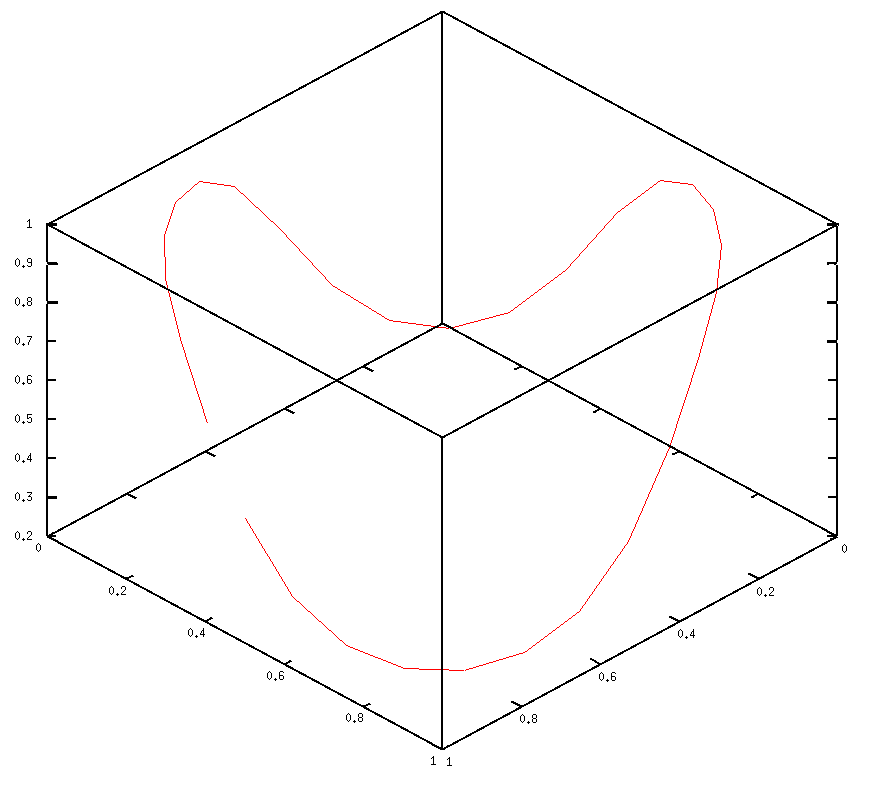
\includegraphics[scale=0.5]{img/xor1}
	\end{center}
	\caption{XOR function}
	\label{fig:xor1}
\end{figure}

\begin{figure}[tb]
	\begin{center}
		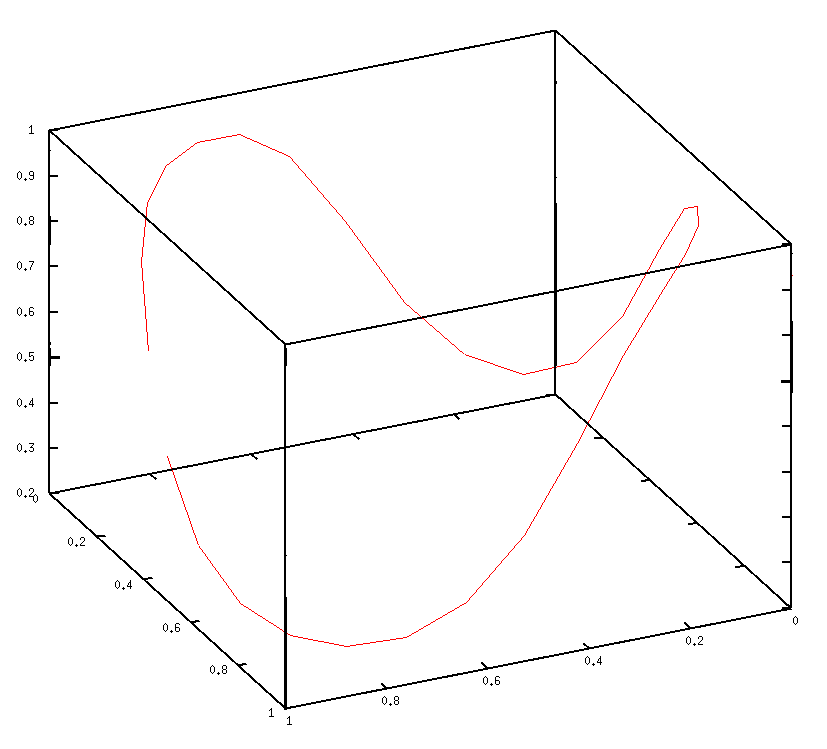
\includegraphics[scale=0.5]{img/xor2}
	\end{center}
	\caption{XOR Function}
	\label{fig:xor2}
\end{figure}

\begin{figure}[tb]
	\begin{center}
		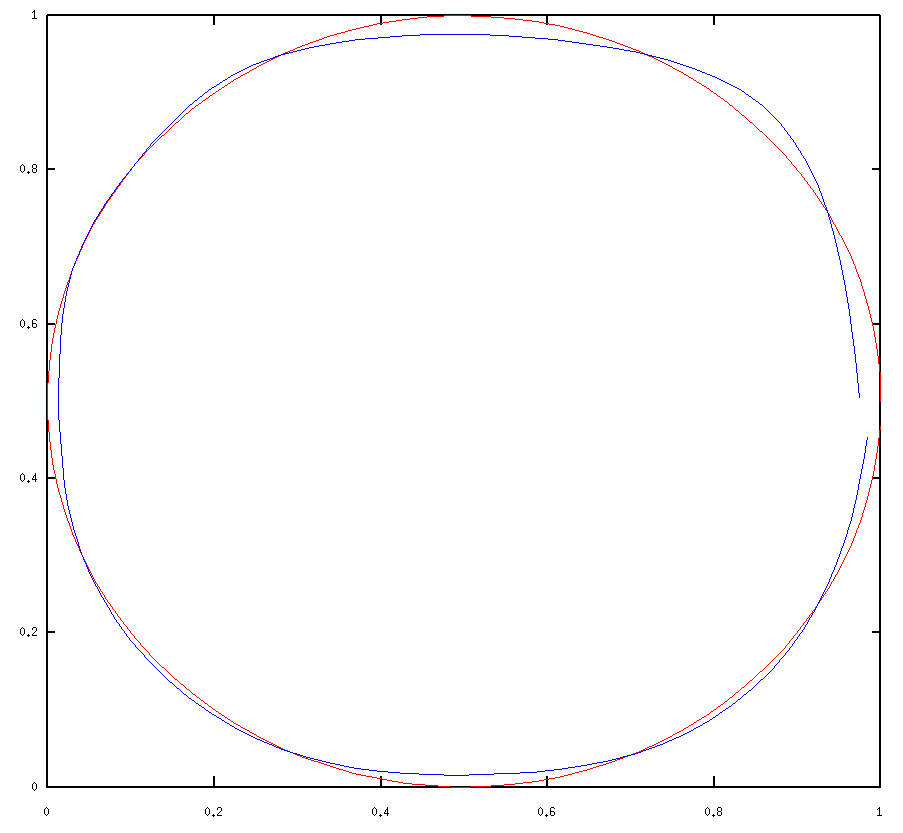
\includegraphics[scale=0.5]{img/circle}
	\end{center}
	\caption{Parametric Circle Function}
	\label{fig:circle}
\end{figure}

\end{document}

% citations:
% weather data